\section{Développement Hardware}
L'architecture du Hardware se présente ainsi :
\begin{figure}[H]
  \centering
  \includegraphics[width=0.75\linewidth]{hardware/architecture}
  \caption{Architecture hardware de PongBoy}
  \label{hard_arc}
\end{figure}
Le circuit est alimenté par 2 piles AAA, et est protégé contre l'inversion
de polarité. Le micro controlleur commande et récupère des infos de l'écran,
de l'haut-parleur, du capteur de luminosité ambiante, et du port multi-joueur.
\newpage

\subsection{Alimentation}
\begin{figure}[H]
  \centering
  \includegraphics[width=0.5\linewidth]{hardware/alim}
  \caption{Alimentation avec protection contre polarité inverse}
  \label{hard_pow}
\end{figure}
La protection d'inversion de polarité est un simple N-MOS qui déconnecte
la masse si la tension est inversée. Cette solution est un dérivé de la méthode
bien connue du P-MOS sur le VCC. Le P-MOS est souvent plus cher et moins
efficace que le N-MOS, ce qui est un problème sur notre circuit basse
consommation.
\newpage

\subsection{Micro Controlleur}
\begin{figure}[H]
  \centering
  \includegraphics[width=0.5\linewidth]{hardware/proc}
  \caption{Micro controlleur PIC18LF25K22 avec attribution des GPIO}
  \label{hard_proc}
\end{figure}
Le micro controlleur utilisé est plutôt limité en GPIO, seulement 3 PORT sont
disponibles, mais 3 PORT complet.
Le bus parallèle de l'écran LCD est entièrement attribué au PORTA.
Les 4 résistances de la dalle tactile sont disposée sur le PORTB, sur les pins
0 à 3, choisies pour leur capacités pull-up, d'interruption externe,
et de mesure analogique.
Le contrôle du rétroéclairage (BCKLGHT) est sur un GPIO avec capacité PWM.
PGC, PGD, TX, RX sont préassignée. Le reste n'a pas besoin de capacité
spécifique.

\begin{figure}[H]
  \centering
  \includegraphics[width=0.25\linewidth]{hardware/prog}
  \caption{Connecteur de programmation du PIC18LF25K22}
  \label{hard_prog}
\end{figure}
Le connecteur de programmation est un connecteur TagConnect. Le layout
du connecteur est celui du PicKit3.
\newpage

\subsection{Écran résistif tactile LCD}
\begin{figure}[H]
  \centering
  \includegraphics[width=0.5\linewidth]{hardware/touch_conn}
  \caption{Connecteur de l'écran tacticle LCD}
  \label{hard_lcd}
\end{figure}
Des MOSFET sont présent pour couper l'alimentation de l'écran.
Étant donné que les MOSFET coupent la masse, il faut s'assurer qu'aucune
des pins de l'écran ne soit à la masse lorsqu'on coupe l'alimentation.
Si une pin se retrouve à la masse, un phénomène appelé \emph{Puit de courant}
se produit, et l'écran arrive à s'alimenter avec cette pin.

Pour ce qui est de la détection et mesure de la pression tactile, le principe
suivant sera utilisé sur les pins XR, XL, YU, YD :
\begin{figure}[H]
  \centering
  \includegraphics[width=0.5\linewidth]{hardware/touch_detect}
  \caption{Détection de la pression tactile}
  \label{hard_touchDetect}
\end{figure}
Pour détecter la pression, on se sert de la dalle tactile comme d'un bouton
poussoir, qui va tirer une pin à la masse. Cela requiert donc une pull-up.

\begin{figure}[H]
  \centering
  \includegraphics[width=0.5\linewidth]{hardware/touch_meas}
  \caption{Mesure de la position de la pression tactile}
  \label{hard_touchMeas}
\end{figure}
Pour mesurer la position de la pression, on se sert du pont présent entre
le X et le Y pour faire la mesure. Ainsi, pour mesurer la position en X, nous
mesurons une des pins Y, et trouvons donc la tension du pont-diviseur X.
Et vice-versa pour la position Y.

\subsection{Périphériques}
\subsubsection{Haut-parleur}
\begin{figure}[H]
  \centering
  \includegraphics[width=0.5\linewidth]{hardware/speaker}
  \caption{Haut-parleur avec MOSFET}
  \label{hard_speaker}
\end{figure}
Le haut-parleur est piloté avec un MOSFET, pour éviter de faire passer du
dans le micro controlleur. Il s'agit d'un haut-parleur inductif, il n'est
donc pas nécessaire d'ajouter de diode ou autre composant pour le fonctionnement
lorsque le MOSFET coupe le circuit.

\subsubsection{Capteur de luminosité ambiante}
\begin{figure}[H]
  \centering
  \includegraphics[width=0.35\linewidth]{hardware/light}
  \caption{Mesure de la lumière ambiante}
  \label{hard_light}
\end{figure}
La mesure de lumière ambiante est réalisée avec une \emph{Light dependant
resistor}. La résistance varie en fonction de la lumière, et cette variation
est mesurée avec un pont-diviseur de tension.
Cette fonctionnalité n'est pour le moment pas du tout implémentée.

\subsubsection{Port multi-joueur}
\begin{figure}[H]
  \centering
  \includegraphics[width=0.5\linewidth]{hardware/multi}
  \caption{Connecteur de communication pour mode multi-joueur}
  \label{hard_multi}
\end{figure}
Un connecteur 3-MOLEX a été choisi, pour avoir une communication full-duplex,
et transmettre une masse commune.
Cette fonctionnalité n'est pour le moment pas du tout implémentée.
\newpage

\section{Boitier mécanique}
\begin{figure}[H]
  \centering
  \includegraphics[width=0.45\linewidth]{mechanical/assembly}
  \caption{Vue éclatée du boîtier complet}
  \label{mech_assembly}
\end{figure}
Le boîtier est composée de deux parties principales : La plaque inférieur,
surlaquelle le circuit imprimé viens se fixer. Et la plaque supérieur, qui
se \emph{clips} sur la plaque inférieur.
Le circuit imprimé est fixé à l'aide de vis M3, et d'inserts filtés.

Un point d'accès aux piles est présent, pour faciliter le changement de piles.
Un stylet a été pensé, pour éviter que l'utilisation du doigt pour le tactile
ne bloque la visibilité de l'écran. Il permet également une utilisation plus
précise du tactile. Le stylet est inspiré de celui d'une \emph{Nintendo DS}.
\begin{figure}[H]
  \centering
  \includegraphics[width=0.45\linewidth]{mechanical/dimensions}
  \caption{Dimensions d'encombrement du bôitier}
  \label{mech_dimensions}
\end{figure}
\newpage

\section{Développement Firmware}
\begin{figure}[H]
  \centering
  \includegraphics[width=\linewidth]{firmware/architecture}
  \caption{Architecture firmware}
  \label{firm_arc}
\end{figure}
Le firmware est découpé en plusieurs modules s'occupant chacun d'un élément
ou d'une partie du PongBoy spécifique :
\begin{itemize}
  \item le LCD driver s'occupe d'afficher sur l'écran, et de gérer le
  rétroéclairage
  \item TouchScreen s'occupe de détecter une pression sur l'écran, et
  de mesurer la position de cette pression pour la transmettre plus loin
  \item Display s'occupe de rafraîchir l'affichage toutes les $30ms$, il
  est informé des changement de menu vers sous-menu, ou vers le jeu
  \item PongBoy controller est une \emph{Factory}, il contient simplement
  tous les controlleurs de la console, comme Display ou Game Controller.
  Il s'occupe également de la mise en veille de la console.
  \item Menu Controller et Game Controller font le lien entre les
  commandes de l'utilisateur, et le menu ou jeu correspondant
  \item Les \emph{GameObjects} Ball et Paddle sont les balles et
  raquette du jeu Pong
\end{itemize}

Le liens entre tout ces modules est le gestionnaire d'évenement XF.
Chaque module peut envoyer un évenement dans la file d'attente de XF, ou
programmer un timer qui transmettera un évenement.
Cette file d'attente est vidée progressivement, et les évenements qui en sortent
sont retransmis à tous les modules, qui modifieront leur comportement selon
l'évenement. Un exemple simple : Le jeu se ferme lorsqu'il reçoit l'évenement
GameOver.

\subsection{TouchScreen}
\begin{figure}[H]
  \centering
  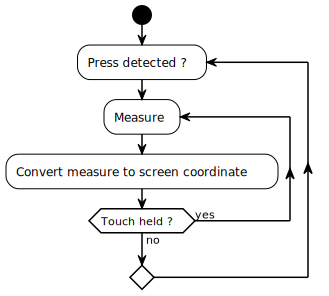
\includegraphics[width=0.5\linewidth]{firmware/touchscreen}
  \caption{Diagramme d'activité du TouchScreen}
  \label{firm_touch}
\end{figure}
La détection de la pression et la méthode de mesure est détaillée au
point 2.1.3.
Le TouchScreen ne mesure que quand une pression est détectée. Les mesures
sont espacées entre elles à l'aide d'un timer.
À la fin de chaque conversion, le TouchScreen envoie un évenement signalant
une nouvelle mesure.
L'interruption externe du tactile permet de transmettre des évenement
\emph{Press} et \emph{Release}.
\newpage

\subsection{Mise en veille}
\begin{figure}[H]
  \centering
  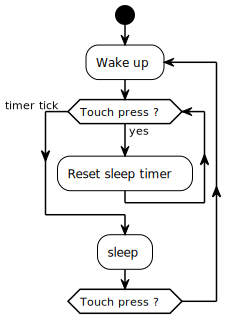
\includegraphics[width=0.5\linewidth]{firmware/pongboy}
  \caption{Diagramme d'activité du PongBoy - fonction veille}
  \label{firm_sleep}
\end{figure}
La mise en veille est gérée avec un timer de XF de $20s$. À chaque
appui sur l'écran tactile, le timer est supprimé et un nouveau est relancé.
\newpage

\subsection{Contrôleurs}
\subsubsection{Pong Controller}
\begin{figure}[H]
  \centering
  \includegraphics[width=0.5\linewidth]{firmware/pong}
  \caption{Diagramme d'activité du Pong Controller}
  \label{firm_pong}
\end{figure}
Le contrôleur de jeu différencie deux états, en jeu et dans le menu.
Lorsqu'on est dans le menu, le jeu ne fais rien.
Lorsqu'on est en jeu, un timer est lancé pour gérer la physique du jeu.
L'affichage du jeu est découplé de ce contrôleur, l'afficheur sait simplement
qu'on est en jeu, et il affiche les objets du jeux sur l'écran toutes les $30ms$.

\subsubsection{Menu Controller}
Le contrôleur de menu fonctionne de manière similaire au pong, sans la partie
jeu. Il comprend des états de sous-menu.
\newpage

\subsection{Paddle}
\begin{figure}[H]
  \centering
  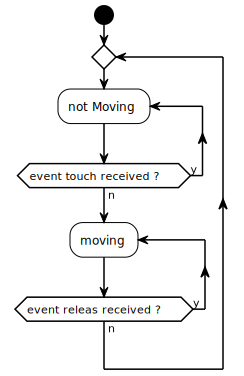
\includegraphics[width=0.5\linewidth]{firmware/paddle}
  \caption{Diagramme d'activité du Paddle}
  \label{firm_paddle}
\end{figure}
La gestion du mouvement du Paddle joueur est découplée du contrôleur de jeu.
Le contrôleur de jeu transmet les évenements au Paddle.
Si une pression sur l'écran a été détectée, le Paddle va checker si la pression
est sur la partie du haut ou du bas de l'écran, et va modifier sa vitesse
en adéquation.
